\section{Введение}
	\subsection{О лаборатории}
	
		
	\begin{frame}
		\frametitle{ФИЦ ИУ РАН}
		\begin{center}
			
\includegraphics[width=0.35\textwidth]{misc/logos/frccsc.png}
		\end{center}
		
		\par\bigskip
		\scriptsize
		Федеральный исследовательский центр <<Информатика и управление>> Российской Академии Наук "--- ведущая организация Российской Федерации, специализирующаяся в научных исследованиях в области информатики и управления.
		
		\textbf{Структурные подразделения:}
		\begin{itemize}
			\item Институт проблем информатики РАН (большие данные, информационная безопасность).
			\item Вычислительный центр РАН (машинное обучение, математическое моделирование).
			\item Институт системного анализа РАН (искусственный интеллект, системный анализ в экономике).
		\end{itemize}
		
		\textbf{Базовые кафедры:}
		\begin{itemize}
			\item ФУПМ МФТИ (<<Системные исследования»>> и <<Интеллектуальные системы>>).
			\item ВМК МГУ (<<Информационной безопасности>>).
			\item МГТУ, МИРЭА, МАИ.
		\end{itemize}
	\end{frame}

	\begin{frame}
		\frametitle{Отдел <<Интеллектуальные динамические системы и когнитивные исследования>>}
		
		\begin{columns}
			\begin{column}{0.7\textwidth}
				Основные направления исследований:
				\begin{itemize}
					\item Искусственный интеллект.
					\item Информационный поиск и анализ текстов (компьютерная лингвистика, психолингвистика, текстовая аналитика).
					\item Системы принятия решений (мультиможножества).
					\item Медицинские экспертные системы.
					\item Робототехнические системы (управление, обучение, планирование).
					\item Компьютерное когнитивные моделирование (модели когнитивных функций, многоагентные системы).
				\end{itemize}
				\par\bigskip
				45 научных сотрудников и инженерных специалистов, 4 доктора наук, 16 кандидатов наук.
			\end{column}
			\begin{column}{0.3\textwidth}
				\centering
				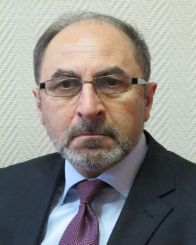
\includegraphics[width=0.4\textwidth]{misc/photos/gs}
				\par\smallskip
				\tiny
				Осипов Геннадий Семенович, зам. дир. ФИЦ ИУ РАН, проф., д.ф.-м.н., президент Российской ассоциации искусственного интеллекта (РААИ)
				\par\medskip
				
\includegraphics[width=0.4\textwidth]{misc/logos/exactus_logo.png}
				\par\medskip
				
\includegraphics[width=0.4\textwidth]{misc/logos/logo_like.png}
				\par\medskip
				
\includegraphics[width=0.4\textwidth]{misc/logos/logo_patent.png}

			\end{column}
		\end{columns}
	\end{frame}

	\begin{frame}
		\frametitle{Группа когнитивного компьютерного\\моделирования}
		\small
		\begin{columns}
			\begin{column}{0.5\textwidth}
				\vspace{-10pt}
				\begin{itemize}
					\item \textbf{Осипов Геннадий Семенович, д.ф.-м.н.},
					\item \textbf{Чудова Наталья Владимировна, к.псих.н.},
					\item \textbf{Кузнецова Юлия Михайловна, к.псих.н.},
					\item \textbf{Панов Александр, к.ф.-м.н.},
					\item Киселев Глеб, асп. ИСА РАН,
					\item Скрыник Алексей, асп. ИСА РАН,
					\item Ковалев Алексей, асп. ВШЭ,
					\item студенты SLabAI.
				\end{itemize}
			\end{column}
			\begin{column}{0.5\textwidth}
				Основные направления исследований:
				\begin{itemize}
					\item Моделирование картины мира человека.
					\item Моделирование когнитивных функций человека с учетом психологических и нейрофизиологических данных.
					\item Планирование поведения и целеполагание.
					\item Обучение и логический вывод в картине мира.
					\item Групповое и коалиционное поведение, распределение ролей.
				\end{itemize}
			\end{column}
		\end{columns}		
	\end{frame}	
	
	\begin{frame}
		\frametitle{Кратко о себе}
		\scriptsize
		\begin{columns}
			\begin{column}{0.85\textwidth}
				\textbf{Панов Александр Игоревич, к. ф.-м. н.}
				\begin{itemize}
					\item Выпускник НГУ и МФТИ.
					\item Старший научный сотрудник отдела <<Интеллектуальные динамические системы и когнитивные исследования>> ФИЦ ИУ РАН.
					\item Научный сотрудник и доцент ФКН ВШЭ.
					\item Доцент кафедры системных исследований Московского физико-технического института (МФТИ).
					\item Член Российской ассоциации искусственного интеллекта (РААИ).
					\item Член Сообщества биологически инспирированных когнитивных архитектур (BICA Society).
					\item Участие в организации Международной конференции по биологически инспирированным когнитивным архитектурам (BICA-2016 --- Нью-Йорк, BICA-2017 --- Москва), Международной школы по биологически инспирированным когнитивным архитектурам (Fierces on BICA, Москва) и школы молодых ученых по ИИ (ISyT 2017, Санкт-Петербург).
					\item Член редколлегии журнала Biologically Inspired Cognitive Architectures.					
					\item Руководитель проектов РФФИ мол\_а, мол\_а\_дк, офи\_м.
					\item Лауреат медали РАН для молодых ученых за 2017 год.
					\item Ментор студенческой лаборатории по ИИ (SLabAI).
				\end{itemize}
			\end{column}
			
			\begin{column}{0.15\textwidth}
				\centering
				\includegraphics[width=\textwidth]{misc/logos/ras.png}
				\vspace{7pt}
				
\includegraphics[width=\textwidth]{misc/logos/frccsc.png}
				\vspace{7pt}
				\includegraphics[width=0.7\textwidth]{misc/logos/isa.png}
				\vspace{7pt}
				\includegraphics[width=0.5\textwidth]{misc/logos/raai.png}
				\vspace{7pt}
				
\includegraphics[width=0.5\textwidth]{misc/logos/hse.png}
				\vspace{7pt}
				\includegraphics[width=\textwidth]{misc/logos/mipt.jpg}
				\vspace{5pt}
				\includegraphics[width=\textwidth]{misc/logos/BICA.png}
				\vspace{5pt}
				\includegraphics[width=0.7\textwidth]{misc/logos/slabai3.png}
			\end{column}
			
		\end{columns}
	\end{frame}
		
	\subsection{Психологические идеи}	
	\begin{frame}
		\frametitle{Когнитивные науки}

		\begin{center}
			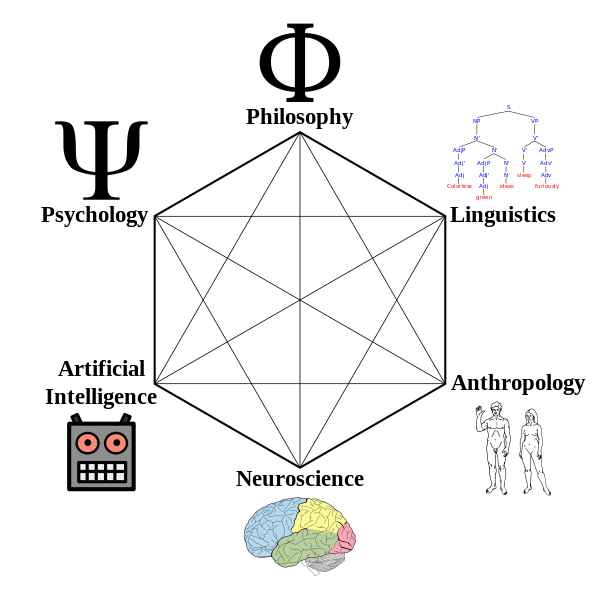
\includegraphics[width=0.3\textwidth]{cogsci.png}
		\end{center}
		
		Когнитивная наука (лат. cognitio <<познание>>) - междисциплинарное научное направление изучающее психику, разум (mind) человека и реализующие его процессы.
		\par\medskip
		Схожие направления в Европе и Америке: \textbf{Artificial General Intelligence} и \textbf{Сommon model of cognition}.
	\end{frame}

	\begin{frame}
		\frametitle{Проблема привязки символов}
		
		\begin{center}
			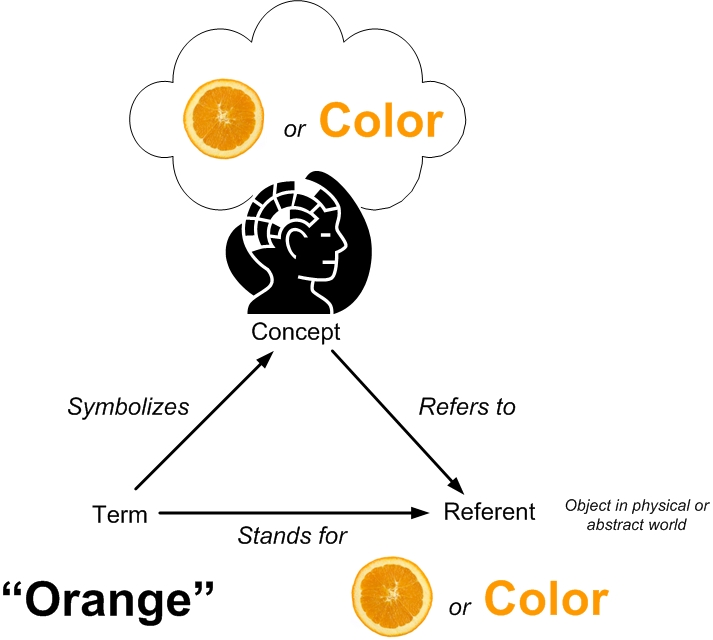
\includegraphics[width=0.3\textwidth]{symb_ground.jpg}
		\end{center}
		\scriptsize
		В оригинале Harnad "--- \textbf{symbol grounding problem} в 1990 г. 
		\par\medskip
		Классические методы искусственного интеллекта являются символьными (логика, множества правил, планирование, обучение). Однако, мышление "--- это больше, чем манипулирование символами.
		\par\medskip
		Особенно эта проблема актуальна в робототехнике (\textbf{symbol anchoring}) "--- система должна обучаться символам на основе своего собственного опыта.
		\nocite{*}
		\printbibliography[keyword={sgp}, resetnumbers=true]
	\end{frame}

	\begin{frame}
		\frametitle{Нейросимвольные вычисления}
		
		\begin{center}
			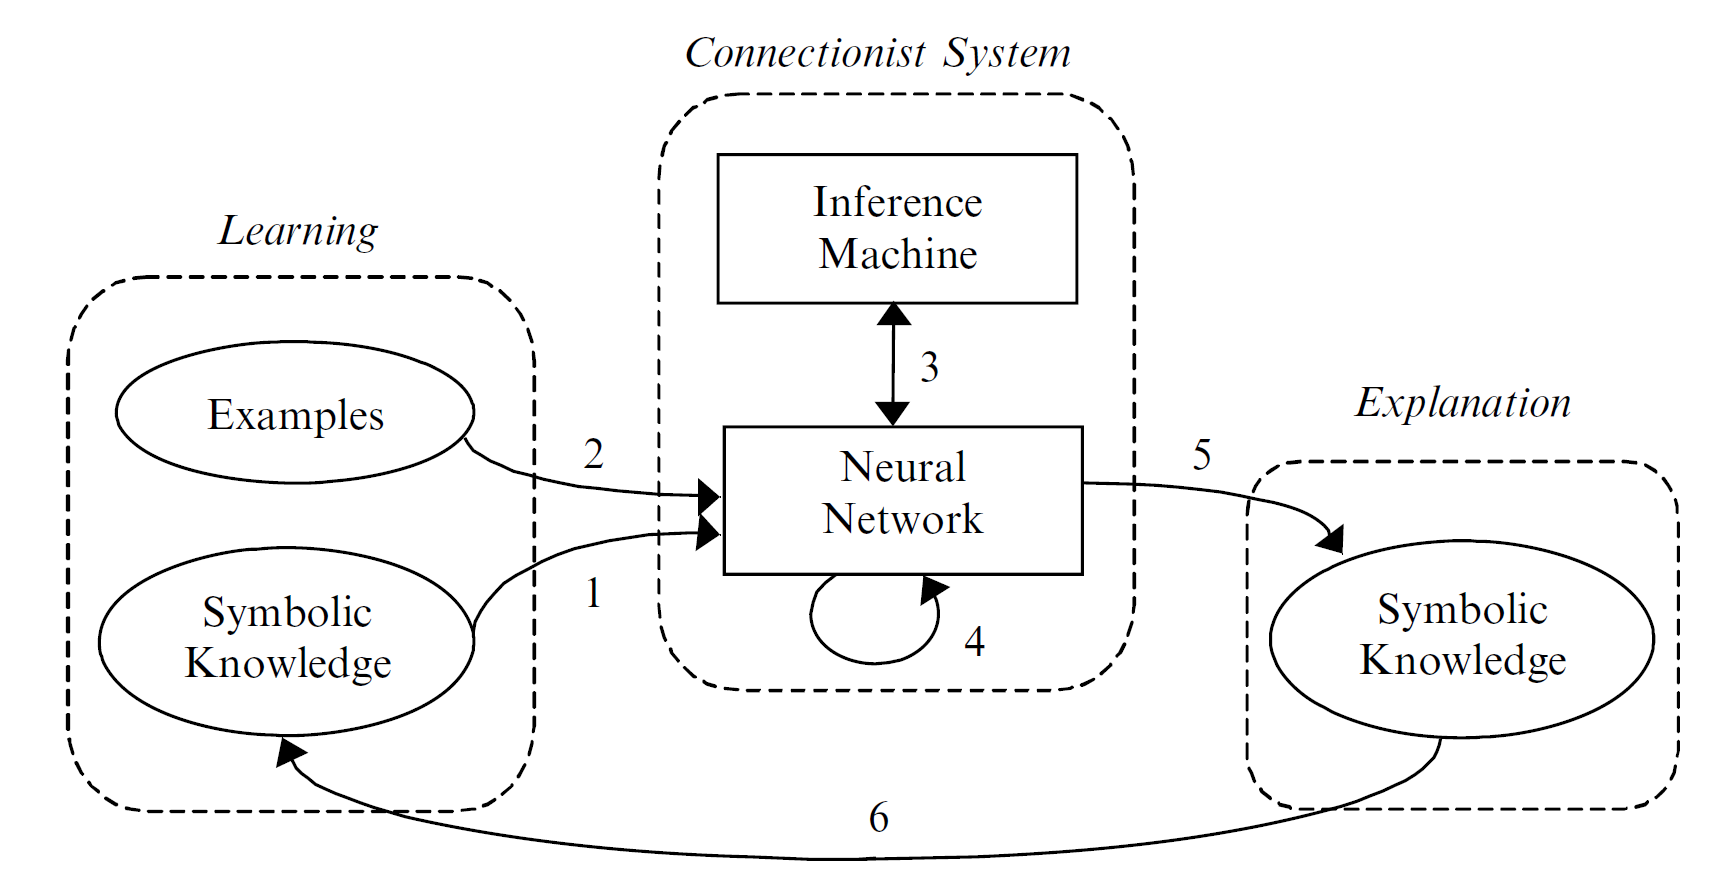
\includegraphics[width=0.3\textwidth]{neuro_symb.png}
		\end{center}
		\textbf{Основная идея}: кодирование символа путем вектора чисел и затем представление этого вектора с помощью связей в ансамбле искусственных нейронов (embending).
		\par\medskip
		\textbf{Основной результат}: путем введения специальных правил по распространению активности по нейронной сети реализованы некоторые простые логические схемы.
		\par\medskip
		\textbf{Основной недостаток}: ограниченная интеграция обучения.
		\nocite{*}
		\printbibliography[keyword={neuro_symb}, resetnumbers=true]
	\end{frame}

	\begin{frame}
		\frametitle{Знак vs. символ}
		\onslide<1->{
		Если прямая интеграция нейронных сетей и символьной обработки работает плохо, то возможно стоит пересмотреть роль \textbf{символа} в общей схеме?
		\par\medskip
		Будем считать, что у символа есть своя структура и у него есть кроме \textbf{номитативной} и другие \textbf{функциональные} роли в реализации когнитивных процессов $\rightarrow$ \textbf{знак}.
		\par\medskip
		Понятие знака как элемента индивидуального знания появилось в концк XIX в.: Пирс, Фреге. Нашло свое отражение в лингвистике, логике, культурологии и \textbf{психологии}.
		}
		\onslide<2->{
			\tikz[baseline]{
			\node[fill=blue!20, rounded corners=5pt, minimum width=330, minimum height = 40] (k1) {
				\begin{minipage}[t][40pt]{330pt}
					\textbf{Идея}: формализовать понятие знака $\rightarrow$ использовать знак в качестве основного структурного элемента системы знаний когнитивного агента $\rightarrow$ построить знаковые модели когнитивных функций.
				\end{minipage}
				
			};
			}
			
		}
		\onslide<1->{
		\vspace{-5pt}
		\nocite{*}
		\printbibliography[keyword={semiotics}, resetnumbers=true]
		}
	\end{frame}
	
	\begin{frame}
		\frametitle{Культурно-исторический подход Выготского}
		\begin{center}
			\includegraphics[width=0.15\textwidth]{misc/photos/vygotsky.jpg}
		\end{center}
		\scriptsize
		Теория происхождения и развития высших психических функций:
		\begin{itemize}
			\item \textbf{Социальная среда} "--- главный источник развития личности.
			\item Овладение культурой, способами поведения и мышления.
			\item Развитие когнитивных функций происходит в первую очередь через использование ребенком \textbf{<<психологических орудий>>}, путем овладения системой знаков-символов, таких как язык, письмо, счет.
			\item Внешняя деятельность, когда культурные средства имеют предметный вид, по мере отработки сворачивается (\textbf{интериоризуется}) во внутренний план.
			\item На первом этапе внешней деятельность ребенок все делает в \textbf{сотрудничестве} со взрослыми, <<зона ближайшего развития>>.
			\item Развитие - не ровно-постепенный, а \textbf{стадиальные} процесс.
			\item Сознание развивается через \textbf{диалог}: диалог ребенка со взрослым либо диалог взрослого со взрослым.
		\end{itemize}
		\end{frame}
		
		\begin{frame}
		\frametitle{Теория деятельности Леонтьева}
		\begin{columns}
		\begin{column}{0.4\textwidth}
			\includegraphics[width=0.8\textwidth]{misc/psycho/activity.pdf}			
		\end{column}
		\begin{column}{0.6\textwidth}
			\begin{center}
				\includegraphics[width=0.17\textwidth]{misc/photos/leontyev.jpg}
			\end{center}
			Основные положения:
			\begin{itemize}
				\item Поведение человека - это двойная иерархическая структура мотивы-цели и действия-операции.
				\item Деятельность – это активный, целенаправленный процесс.
				\item Действия человека предметны; их цели носят социальный характер.
				\item Сознание и деятельность неразрывно связаны.
			\end{itemize}
		\end{column}
		\end{columns}
	\end{frame}

	\begin{frame}
		\frametitle{Знак как орудие психической деятельности}
		\begin{center}
			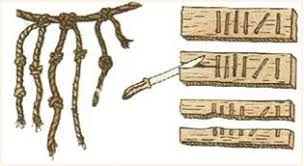
\includegraphics[width=0.4\textwidth]{link.jpg}
		\end{center}

		\begin{itemize}
			\item Знак - это искусственно созданный человеком стимул, средство для управления своим поведение и поведением других.
			\item История развития человечества - это история развития знака: чем более развита система знаков в поколении, тем более развиты высшие психические функции.
			\item Знаки: наскальный рисунок, приметы, жесты, речь, ноты и т.д.
		\end{itemize}
	\end{frame}

	\begin{frame}
		\frametitle{Прикладная семиотика}
		\begin{center}
			\includegraphics[width=0.2\textwidth]{signs/ru/sign-frame.png}
		\end{center}
		\vspace{-15pt}
		\scriptsize
		Семиотические базы знаний:
		\begin{itemize}
			\item \textbf{Именованность}: информационная единица, которая претендует на то, чтобы называться знанием, должна иметь некоторую собственную метку - имя.
			\item \textbf{Структурированность}: информационная единица должна обладать своей внутренней структурой.
			\item \textbf{Принцип матрешки}: знаки за счет связей наследования как бы вкладываются друг в друга, обеспечивая описание сущностей на различных уровнях.
			\item \textbf{Связность}: знаки благодаря различным отношениям объединяются в сеть.
			\item \textbf{Активность}: в сетях знаков становится возможной реализация принципа <<активизация знаний - источник активизации процедур>>.
			\item \textbf{Рефлексивность}: появление метауровня позволяет системе рассуждать о самой себе, о характере имеющейся у нее информации об окружающем мире.
		\end{itemize}
		\vspace{-5pt}
		\nocite{*}
		\printbibliography[keyword={apply}, resetnumbers=true]
	\end{frame}

	\begin{frame}
		\frametitle{Когнитивные архитектуры}
		\begin{center}
			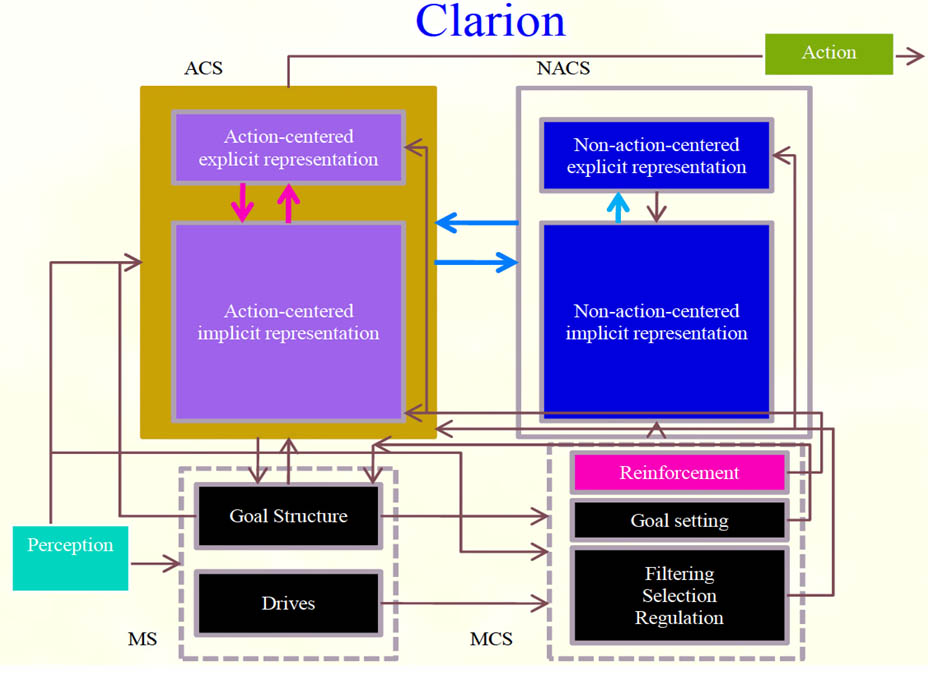
\includegraphics[width=0.3\textwidth]{clarion.jpg}
			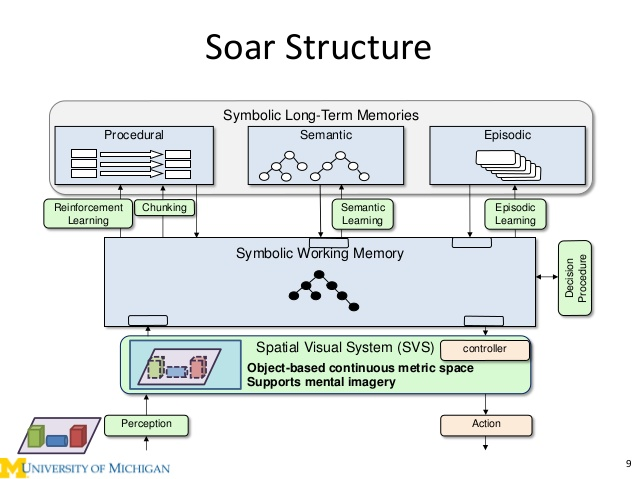
\includegraphics[width=0.3\textwidth]{soar.jpg}
		\end{center}
		\scriptsize
		Недостатки современных когнитивных архитектур:
		\begin{itemize}
			\item Концептуальная нерешенность проблемы привязки символов (symbol grounding problem) - CLARION
			\item Отсутствие деятельностной модели поведения системы - реализация только некоторых когнитивных аспектов
			\item Иерархичность представления знаний (4D/RCS)
			\item Возможность реализации иерархического планирования
			\item Реализация обучения концептуальным знаниям - Cognitive Mario
			\item Моделирование рефлексивного поведения
		\end{itemize}
		\vspace{-5pt}
		\nocite{*}
		\printbibliography[keyword={symbgrnd}, resetnumbers=true]
	\end{frame}